%To compute the Pedersen hash of a message $M$, that is, expression \ref{eq-ped}, the idea is to compute each term separately and add them together. 
In the following circuit \textsc{pedersen hash}, we have depicted the circuit used to compute the Pedersen hash of a message $M$ described in equation \ref{eq-ped}. Each \textsc{multiplication} box returns a term of the sum. 
%that takes, per bit, that many constraints (of a circuit). 

\begin{figure}[h]
	\centering
	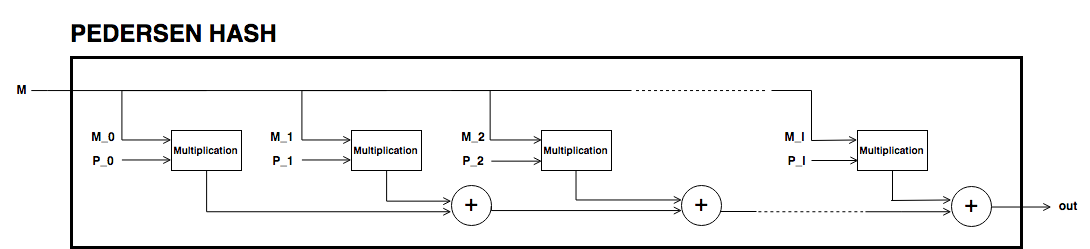
\includegraphics[scale=0.4]{figures/pedersen-hash.png}
	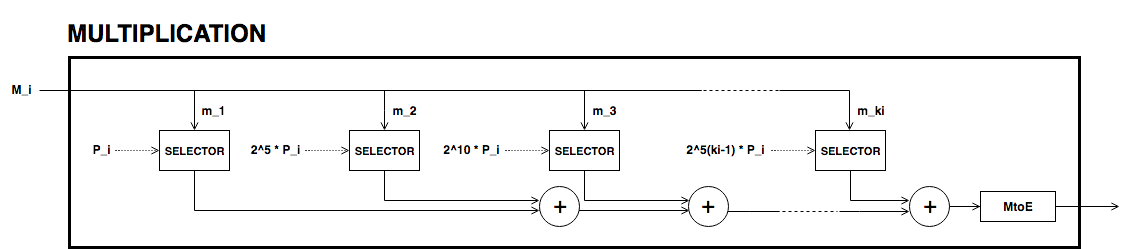
\includegraphics[scale=0.4]{figures/pedersen-multiplication.png}
\end{figure}

As the set of generators are fixed, we can precompute its multiples and use 4-bit lookup windows to select the right points. This is done as shown in the circuit called \textsc{selector}. This circuit receives 4-bit chunk input and returns a point. The first three bits are used to select the right multiple of the point and last bit decides the sign of the point. The sign determines if the $x$-coordinate should be taken positive or negative, as with \red{twisted Edwards curves}, negating a point corresponds to the negation of its first coordinate [REF]. 

\begin{figure}[h]
	\centering
	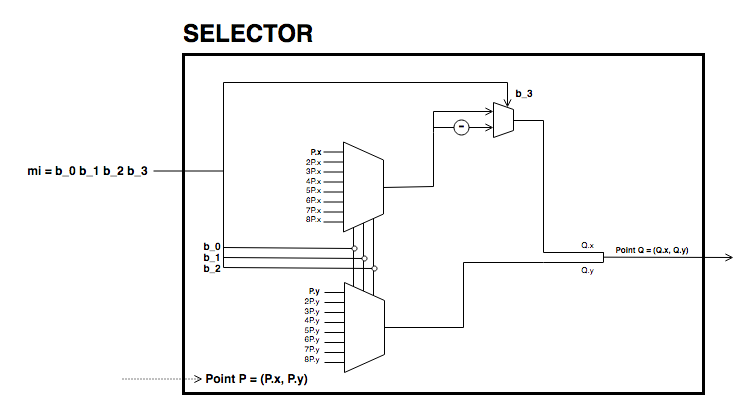
\includegraphics[scale=0.5]{figures/pedersen-multiplication-selector.png}
\end{figure}

